\documentclass[tikz]{standalone}

\usepackage{tikz}
\usetikzlibrary{trees}
\usetikzlibrary{shapes}
\usetikzlibrary{positioning}
\usetikzlibrary{arrows.meta}

\tikzset{
    mynode/.style = {circle, ultra thick, draw=black, align=center,fill=yellow!30,font=\ttfamily\bfseries\Large,text=black},
    mynoder/.style = {circle, ultra thick, draw=black, align=center,fill=red!30,font=\ttfamily\bfseries\Large,text=black},
    mynodeb/.style = {circle, ultra thick, draw=black, align=center,fill=blue!30,font=\ttfamily\bfseries\Large,text=black},
    mynodeg/.style = {circle, ultra thick, draw=gray, align=center,fill=gray!05,font=\ttfamily\bfseries\Large,text=gray!20},
    mynodegr/.style = {circle, ultra thick, draw=gray, align=center,fill=gray!05,font=\ttfamily\bfseries\Large,text=red},
    edgen/.style = {-,ultra thick,black},
    edger/.style = {-,ultra thick,red},
    edgeb/.style = {-,ultra thick,blue},
    edgeg/.style = {-,ultra thick,gray},
    edgegd/.style = {-,ultra thick,brown,dashed}, % back
    edgevd/.style = {-,ultra thick,violet,dotted}, % forward
    edgexd/.style = {-,ultra thick,blue,densely dotted}, % traversal
    every picture/.style={/utils/exec={\ttfamily\bfseries}},
    every picture/.style={font issue=\ttfamily\bfseries},
    font issue/.style={execute at begin picture={#1\selectfont}}
}

\newcommand{\R}[1]{\textcolor{red}{#1}}
\newcommand{\B}[1]{\textcolor{violet}{#1}}

\begin{document}

%%%% 1
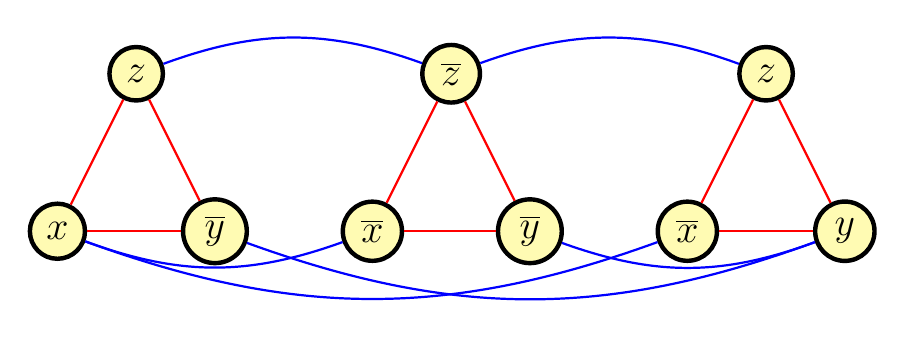
\begin{tikzpicture}[scale=1.00,transform shape]
\node[mynode] at (0.0, 0.0) (x1) {$x$};
\node[mynode] at (2.0, 0.0) (y1) {$\overline{y}$};
\node[mynode] at (4.0, 0.0) (x2) {$\overline{x}$};
\node[mynode] at (6.0, 0.0) (y2) {$\overline{y}$};
\node[mynode] at (8.0, 0.0) (x3) {$\overline{x}$};
\node[mynode] at (10.0, 0.0) (y3) {$y$};
\node[mynode] at (1.0, 2.0) (z1) {$z$};
\node[mynode] at (5.0, 2.0) (z2) {$\overline{z}$};
\node[mynode] at (9.0, 2.0) (z3) {$z$};
%
\draw[edger, thick,-] (x1) edge node {} (y1);
\draw[edger, thick, -] (y1) edge node {} (z1);
\draw[edger, thick, -] (z1) edge node {} (x1);
\draw[edger, thick, -] (x2) edge node {} (y2);
\draw[edger, thick, -] (y2) edge node {} (z2);
\draw[edger, thick, -] (z2) edge node {} (x2);
\draw[edger, thick, -] (x3) edge node {} (y3);
\draw[edger, thick, -] (y3) edge node {} (z3);
\draw[edger, thick, -] (z3) edge node {} (x3);
\draw[edgeb, bend left = 20, thick, -] (z1) edge node {} (z2);
\draw[edgeb, bend left = 20, thick, -] (z2) edge node {} (z3);
\draw[edgeb, bend right = 20, thick, -] (x1) edge node {} (x2);
\draw[edgeb, bend right = 20, thick, -] (x1) edge node {} (x3);
\draw[edgeb, bend left = 20, thick, -] (y3) edge node {} (y2);
\draw[edgeb, bend left = 20, thick, -] (y3) edge node {} (y1);
\end{tikzpicture}

%%%% 2
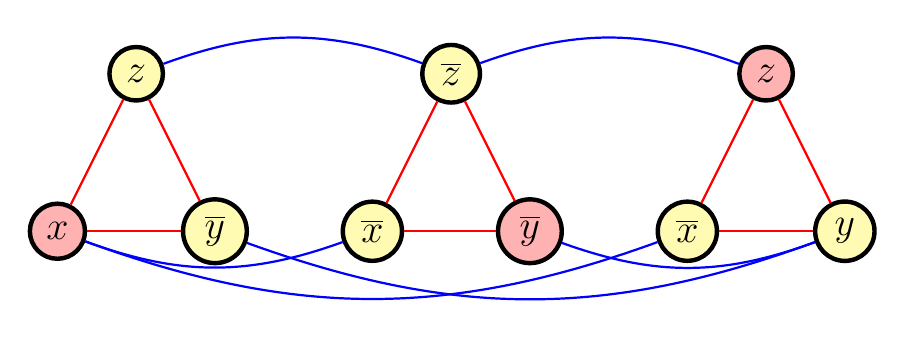
\begin{tikzpicture}[scale=1.00,transform shape]
\node[mynoder] at (0.0, 0.0) (x1) {$x$};
\node[mynode] at (2.0, 0.0) (y1) {$\overline{y}$};
\node[mynode] at (4.0, 0.0) (x2) {$\overline{x}$};
\node[mynoder] at (6.0, 0.0) (y2) {$\overline{y}$};
\node[mynode] at (8.0, 0.0) (x3) {$\overline{x}$};
\node[mynode] at (10.0, 0.0) (y3) {$y$};
\node[mynode] at (1.0, 2.0) (z1) {$z$};
\node[mynode] at (5.0, 2.0) (z2) {$\overline{z}$};
\node[mynoder] at (9.0, 2.0) (z3) {$z$};
%
\draw[edger, thick,-] (x1) edge node {} (y1);
\draw[edger, thick, -] (y1) edge node {} (z1);
\draw[edger, thick, -] (z1) edge node {} (x1);
\draw[edger, thick, -] (x2) edge node {} (y2);
\draw[edger, thick, -] (y2) edge node {} (z2);
\draw[edger, thick, -] (z2) edge node {} (x2);
\draw[edger, thick, -] (x3) edge node {} (y3);
\draw[edger, thick, -] (y3) edge node {} (z3);
\draw[edger, thick, -] (z3) edge node {} (x3);
\draw[edgeb, bend left = 20, thick, -] (z1) edge node {} (z2);
\draw[edgeb, bend left = 20, thick, -] (z2) edge node {} (z3);
\draw[edgeb, bend right = 20, thick, -] (x1) edge node {} (x2);
\draw[edgeb, bend right = 20, thick, -] (x1) edge node {} (x3);
\draw[edgeb, bend left = 20, thick, -] (y3) edge node {} (y2);
\draw[edgeb, bend left = 20, thick, -] (y3) edge node {} (y1);
\end{tikzpicture}


\end{document}